\documentclass[12pt]{article}
\usepackage{mathematics}

\begin{document}

\begin{mdframed}
  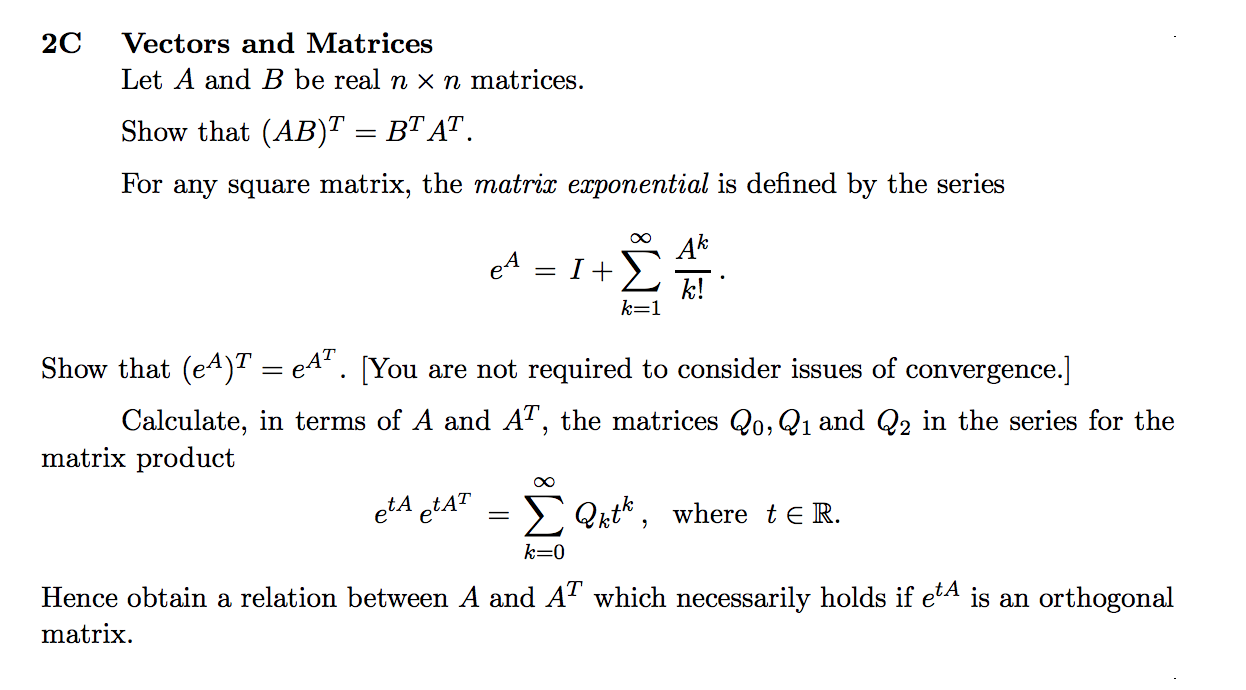
\includegraphics[width=400pt]{img/misc--cambridge-1a-2017-1-2c.png}
\end{mdframed}

\begin{claim*}
  $(AB)^T = B^TA^T$
\end{claim*}

\begin{proof}
  Let $i, j \in \{1, \ldots, n\}$. Then
  \begin{align*}
    \((AB)^T\)_{ij} &= (AB)_{ji}
                   = \sum_{l=1}^n A_{jl}B_{li}
                   = \sum_{l=1}^n (A^T)_{lj}(B^T)_{il}
                   = (B^TA^T)_{ij}
  \end{align*}
\end{proof}

\begin{lemma*}
  $(A^k)^T = (A^T)^k$.
\end{lemma*}

\begin{proof}
  Note that $(A^m)^T(A^T)^n = (AA^{m-1})^T(A^T)^n = (A^{m-1})^T(A^T)^{n+1}$. By iterating this
  formal manipulation $k$ times, we have $(A^k)^T = (A^k)^T(A^T)^0 = (A^0)^T(A^T)^k = (A^T)^k$.
\end{proof}

\begin{claim*}
  $(e^A)^T = e^{(A^T)}$
\end{claim*}

\begin{proof}
  Note that $(e^A)_{ij} := \sum_{k=0}^\infty \frac{(A^k)_{ij}}{k!}$, where $A^0 := I$ and
  $0! := 1$.  Therefore
  \begin{align*}
    \((e^A)^T\)_{ij} = \sum_{k=0}^\infty \frac{((A^k)^T)_{ij}}{k!}
                    = \sum_{k=0}^\infty \frac{((A^T)^k)_{ij}}{k!}
                    = \(e^{(A^T)}\)_{ij} .
  \end{align*}
\end{proof}

\end{document}
